\documentclass{beamer}

\usepackage{amsmath}
\usepackage{physics}
\usetheme{Boadilla}

%Information to be included in the title page:
\title{Qiskit Crash Course Workshop}
\subtitle{YuQC Fall Fest}
\author{Ben McDonough and Alex Deters}
\date{2022}

\begin{document}

\frame{\titlepage}

\section{Representing Quantum States}
\begin{frame}
\frametitle{Linear Algebra Concepts}
 Spanning set: Let $V$ be a vector space and $\{\vec s_1,...,\vec s_N\} = S$ be a set of vectors spanning $V$. Then if $\vec v \in V$, 
$$
\vec v = \sum_{i=1}^N c_i \vec s_i
$$
for some coefficients $c_i$.
Orthogonal: Two vectors $\vec v_1$ and $\vec v_2$ are called orthogonal if their inner product is zero: $$
\vec v_1 \cdot \vec v_2 = 0
$$
Normal: A vector $\vec v$ is called normal if it has a norm of one:
$$
\Vert \vec v \Vert = \sqrt{\vec v \cdot \vec v} =  1
$$
Basis: an orthogonal, normal (orthonormal) spanning set is called a basis
\end{frame}
\begin{frame}
\frametitle{Linear Algebra Contd.}
A map $T(\vec v)$ is called linear if
$$
T\qty(\sum_{i=1} c_i \vec v_i) = \sum_{i=1}c_i T(\vec v_i)
$$
If $\vec v$ is an arbitrary vector and $B$ is a basis for $V$, then combining the definition of spanning
$$
T(\vec v) = \sum_{i}^N c_i T(\vec b_i)
$$
In this way, $T$ is uniquely specified by defining $T(\vec b_i)$ for all $b_i$. 
A vector $\vec v$ is called an eigenvector of $T$ with eigenvalue $\lambda$ if
$$
T(\vec v) = \lambda \vec v
$$
Every linear map has as a representation as a matrix.
\end{frame}
\begin{frame}
\frametitle{From Matrices to Kets}
Quantum states are represented in terms of distinguishable basis states
\begin{example}
A coin can be in two states: heads or tails. Imagine representing heads with $\begin{pmatrix}1 \\ 0 \end{pmatrix}$ and tails with $\begin{pmatrix}0 \\ 1 \end{pmatrix}$. Then a weighted coin in heads with probability $\alpha$ and tails with probability $\beta$ could be represented as $\begin{pmatrix} \alpha \\ \beta \end{pmatrix}$, with $\alpha + \beta = 1$
\end{example}
Another way to represent the basis states in to use bra-ket notation. For instance, say
\begin{align*}
\begin{pmatrix}1 \\ 0 \end{pmatrix} &\dot = \ket{\text{heads}} & \begin{pmatrix} 0 \\ 1 \end{pmatrix} &\dot = \ket{\text{tails}}
\end{align*}
Then the state from before would be $\ket{\text{coin}} = \alpha \ket{\text{heads}}+\beta \ket{\text{tails}}$
\end{frame}
\begin{frame}
\frametitle{Overlaps and Dot Product}
We define the overlap of two states as $\braket{a}{b}$
\begin{itemize}
\item Since the states $\ket{\text{heads}}$ and $\ket{\text{tails}}$ are distinguishable, we say they do not overlap. We require that the overlap of a state with itself is always one:
$$\braket{\text{tails}}{\text{heads}} = 0 \ \ \text{and} \ \ \braket{\text{tails}}{\text{tails}} = 1
$$
\item This means that $\ket{\text{tails}}$ is a linear map such that $\bra{\text{tails}}\mqty(1 \\ 0) = 0$ and $\bra{\text{tails}}\mqty(0 \\ 1) = 1$. In matrix form, the bra is the transpose of the ket:
$$
\bra{\text{tails}} \dot= \mqty(1 & 0) = \mqty(1 \\ 0)^\top \dot = \ket{\text{tails}}^\top
$$
This is also recognizable as the dot product $\braket{\text{tails}}{\text{heads}} = \ket{\text{tails}} \cdot \ket{\text{heads}}$.
\end{itemize}
\end{frame}
\begin{frame}
\frametitle{Leap to Quantum}
In quantum computing, a single qubit has two possible states, just like the coin: $\ket{0}$ and $\ket{1}$. These states form a basis for the qubit state space.\vspace{.5cm}

States belong to a ``Hilbert Space", so the scalars are complex numbers
\begin{alertblock}{Complex numbers}
\begin{itemize}
\item Complex numbers are written $z = a+bi$, where $i = \sqrt{-1}$
\item The conjugate is defined as $z^\ast \cong a-bi$
\end{itemize}
\end{alertblock}
Therefore an arbitrary qubits state, traditionally represented by $\psi$, can be written 
$$
\ket{\psi} = \alpha \ket{0} + \beta \ket{1}
$$
With $\alpha$ and $\beta$ being complex numbers.
\end{frame}
\begin{frame}
\frametitle{Leap to Quantum Contd.}
Normalization: The Hilbert space is endowed with the norm:
$$
\Vert \ket{\psi} \Vert = \sqrt{\braket{\psi}{\psi}}
$$
The normalization condition requires that $\braket{\psi}{\psi}$ = 1. In matrix form, the transpose is replaced by the adjoint:
$$
\braket{\psi}{\psi} = \mqty(\alpha^\ast & \beta^\ast)\mqty(\alpha \\ \beta) = (\ket{\psi})^\dagger \ket{\psi}
$$
As shown above, the adjoint, or Hermitian conjugate of a matrix is performed by taking the transpose and then conjugating all the matrix elements.
\end{frame}
\section{Measurement}
\begin{frame}
\frametitle{The Borne Rule}
One of the fundamental postulates of quantum mechanics is discrete measurement outcomes.
\begin{example}
\textbf{Stern-Gerlach Experiment} Silver atoms have a magnetic moment determined by the spin of their outermost electron. When silver atoms are passed through a magnetic field, one would expect them to be deflected in random directions corresponding to random spins. The Stern-Gerlach experiment showed that they were only deflected in two directions, corresponding to discrete measurement outcomes.
\end{example}
Take $\ket{\psi} = \alpha \ket 0 + \beta \ket 1$ to be an arbitrary state. Then the probability of measuring $\ket{\psi}$ in the states $\ket 0$ and $\ket 1$ are given by
\begin{align*}
p(0) &= |\braket{0}{\psi}|^2 = |\alpha|^2 & p(1) &= |\braket{1}{\psi}|^2 = |\beta|^2
\end{align*}
\end{frame}
\begin{frame}

\frametitle{Euler's formula}
Let $f(\theta) = \frac{cos(\theta)+i\sin(\theta)}{e^{i\theta}}$
Take the derivative with the product rule: 
$$
f'(\theta) = \frac{e^{i\theta}(-\sin(theta)-i\cos(\theta))+ie^{i\theta}(\cos(\theta)+\sin(\theta))}{e^{2i\theta}} = 0
$$
We have $f'(\theta) = 0$, and so $f(\theta) = C$. Plugging in $\theta = 0$, we see $f(0) = 1$, so
$$
\cos(\theta) + i\sin(\theta) = e^{i\theta}
$$
for all $\theta$. This gives a new way to represent complex numbers:
$$
z = a+bi = \sqrt{a^2+b^2}[\underbrace{\frac{a}{\sqrt{a^2+b^2}}}_{\cos(\theta)}+i\underbrace{\frac{b}{\sqrt{a^2+b^2}}}_{\sin(\theta)}] = |z|e^{i\theta}
$$
Where $|z| = \sqrt{a^2+b^2}$.
\end{frame}
\begin{frame}
\frametitle{The Bloch Sphere}
Multiplying $\ket \psi$ by $e^{i\phi'}$ does not affect the measurement outcome, because
$$
|\bra{\delta}e^{i\phi'}\ket{\psi}|^2 = |e^{i\phi'}|^2|\bra{\delta}\ket{\psi}|^2 = |\bra{\delta}\ket{\psi}|^2 
$$
This makes a complex ``global phase" undetectable. \\
\vspace{.5cm}
Let $\ket \psi = \alpha \ket 0 + \beta \ket 1$. Through Euler's formula, we can write
$
\alpha = ae^{i\phi'}
$
and
$
\beta = be^{i\phi''}
$
, and with this we can factor out the phase to make $\alpha$ real WLOG:
$$
\ket{\psi} = a\ket{0}+be^{i\phi}\ket 1
$$
Where $\phi = \phi'-\phi''$. Then, we require that $\braket{\psi}{\psi} = a^2+b^2 = 1$, so we can use the trig identity $\cos[2](\frac{\theta}{2}) + \sin[2](\frac{\theta}{2}) = 1$ to rewrite
$$
\ket{\psi} = \cos(\frac{\theta}{2})\ket{0}+\sin(\frac{\theta}{2})e^{i\phi}\ket{1}
$$
\end{frame}
\begin{frame}
\frametitle{Bloch Sphere Contd.}
If we imagine a unit sphere with antipodal points corresponding to $\ket{0}$ and $\ket{1}$, then $\ket \psi$ can be represented on this unit sphere with polar angle $\theta$ and azimuthal angle $\phi$ (this was the reason for choosing $\frac{\theta}{2}$):
\begin{figure}
\centering
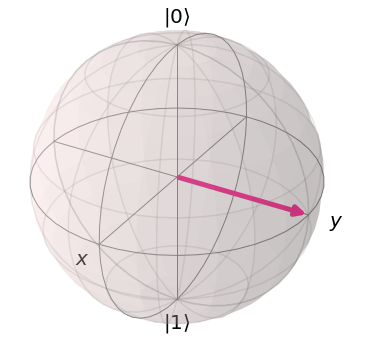
\includegraphics[scale=.4]{scrn-2022-10-04-15-44-49.png}
\caption{Bloch plot for $\theta = \pi$, $\phi = \pi$}
\end{figure}
\end{frame}
\section{Operators}
\begin{frame}
\frametitle{Quantum Operators}
In quantum mechanics, the state changes in time by multiplication by a linear operator $U$.
\begin{block}{note}
$U$ should preserve the norm of states so that probability still makes sense. This means that $\Vert \ket{\delta}\Vert ^2 = \bra{\delta}U^\dagger U \ket{\delta} = \braket{\delta}{\delta}$, so $U^\dagger U = I$. This property is called \textit{unitarity}.
\end{block}
Any single-qubit operator $U$ is defined by $U\ket{0} = c_0\ket{\psi_0}$ and $U\ket{1} = c_1\ket{\psi_1}$. Another way to express this is with outer products:
$$
U = c_0\ketbra{\psi_0}{0}+c_1 \ketbra{\psi_1}{1}
$$
\end{frame}
\begin{frame}
\frametitle{The $X$ gate}
The $X$ gate, or Pauli-$X$ gate, is a common single-qubit gate. This is the gate that flips the $\ket{0} \leftrightarrow \ket{1}$ states. Symbolically, this can be written
$$
X = \ketbra{0}{1} + \ketbra{1}{0} \dot = \mqty(0 & 1 \\ 1 & 0)
$$
The matrix representation can be found in the computational basis by putting the coefficient on $\ketbra{i}{j}$ in the $i^\text{th}$ row and $j^\text{th}$ column of the matrix.\vspace{.5cm}
The eigenstates of this operator form the $X-$basis, and are even combinations of $\ket{0}$ and $\ket{1}$:
\begin{align*}
\mqty(0 & 1 \\ 1 & 0)\mqty(\frac{1}{\sqrt{2}} \\ \frac{1}{\sqrt{2}}) &= \mqty(\frac{1}{\sqrt{2}} \\ \frac{1}{\sqrt{2}}) & \mqty(0 & 1 \\ 1 & 0)\mqty(\frac{1}{\sqrt{2}} \\ -\frac{1}{\sqrt{2}}) &= -\mqty(\frac{1}{\sqrt{2}} \\ -\frac{1}{\sqrt{2}}) 
\end{align*}
\end{frame}
\begin{frame}{The Hadamard Gate}
Another important gate is the Hadamard gate. This gate takes the $Z-$eigenstates to the $X-$ eigenstates, so
\begin{align*}
H\mqty(1 \\ 0) &= \mqty(\frac{1}{\sqrt{2}} \\ \frac{1}{\sqrt{2}}) & H\mqty(0 \\ 1) &= \mqty(\frac{1}{\sqrt{2}} \\ -\frac{1}{\sqrt{2}})
\end{align*}
If we write the $X-$eigenstates as $\ket{+} = \frac{\ket{0}+\ket{1}}{\sqrt{2}}$ and $\ket{-} = \frac{\ket 0-\ket{1}}{\sqrt{2}}$, then we can write the Hadamard matrix as
$$
H = \ketbra{+}{0}+\ketbra{-}{1} = \frac{1}{\sqrt{2}}\qty(\ketbra{0}{0}+\ketbra{0}{1}+\ketbra{1}{0}-\ketbra{1}{1})
$$
In matrix representation,
$$
H \dot = \frac{1}{\sqrt{2}}\mqty(1 & 1 \\ 1 & -1)
$$
\end{frame}

\begin{frame}
\frametitle{State Collapse}
When an operator $M$ is measured, the experimentalist obtains the eigenvalue $\lambda$ and the system collapses into then corresponding eigenvector $\ket{\lambda}$.
\begin{alertblock}{Important!}
    Like the coin in the box, the system is left in a definite state after observation. But don't let this deceieve you--the coin was in a definite but unknown state before measurement, whereas the qubit was not in any definite state at all.
\end{alertblock}
\begin{block}{note}
A Hermitian operator is one such that $M^\dagger = M$. Hermitian operators correspond to physical observable quantities because they have strictly real eigenvalues.
\end{block}
Measurement irreversibly destroys quantum information!
\end{frame}
\begin{frame}
\frametitle{Expectation Values}
A property of Hermitian operators is that they can be written as ``diagonal" in the basis of their eigenvectors. If $M$ is an operator with eigenvectors $\ket{a}$ and $\ket{b}$ with corresponding eigenvalues $a$ and $b$, then
$$
M = a\ketbra{a}{a}+b\ketbra{b}{b}
$$
Given some sort of operator $M$ that we want to find the expectation value of, we can simply compute,
\begin{align*}
    \langle M \rangle_\psi &= \expval{M}{\psi}
\end{align*}
For a Hermitian operator, this means
$$
\langle M \rangle_\psi = \bra{\psi} a\ketbra{a}{a}+b\ketbra{b}{b}\ket{\psi} = a|\braket{a}{\psi}|^2+b|\braket{b}{\psi}|^2 = ap(a)+bp(b)
$$
\end{frame}
\begin{frame}
\frametitle{Entanglement}
This can easily be extended to multiple qubits. Two separate qubit states can be combined using the ``Kronecker product" symbol,
$$
\ket{01}_{AB} = \ket{0}_B \otimes \ket{1}_A
$$
When a multi-qubit state can be written as a Kronecker product, it is called a product state. Operators can also take the form of kronecker products, and they act on their respective subsystems
$$
(X_B \otimes X_A)\ket{0}_B \otimes \ket{1}_A = X_A\ket{0}_A \otimes X_B\ket{1}_B = \ket{1}_B \otimes \ket{0}_A
$$
When states cannot be represented as product states, they are called product states. The canonical example is the first Bell state $\ket{\Phi_0}$:
$$
\ket{\Phi_0} = \frac{\ket{00}+\ket{11}}{\sqrt{2}}
$$
\end{frame}
\end{document}